\documentclass[11pt,letterpaper]{article}
\usepackage[lmargin=1in,rmargin=1in,tmargin=1in,bmargin=1in]{geometry}
\usepackage{../style/homework}
\usepackage{../style/commands}
\setbool{quotetype}{true} % True: Side; False: Under
\setbool{hideans}{false} % Student: True; Instructor: False

% -------------------
% Content
% -------------------
\begin{document}

\homework{16: Due 11/09}{I believe that we do not know anything for certain, but everything probably.}{Christiaan Huygens}

% Problem 1
\problem{10} Suppose at a local grocery store, 8 employees work only in the back of the store, 17 work only in the front of the store, and 9 work in both positions.
	\begin{enumerate}[(a)]
	\item Find the percentage of students that work in the back of the store.
	\item Find the percentage of employees that work in the back of the store or in the front of the store.
	\item Find the percentage of employees that work either in the front or back of the store, but not both. 
	\item Assuming an employee works in the front of the store, what is the probability that they also work in the back of the store?
	\end{enumerate} \pspace

\sol 
\begin{enumerate}[(a)]
\item 
	\[
	P(\text{back})= \dfrac{8 + 9}{34}= \dfrac{17}{34} \approx 0.50
	\]

\item 
	\[
	P(\text{back or front})= \dfrac{8 + 9 + 17}{34}= \dfrac{34}{34} \approx 1.00
	\]

\item 
	\[
	P(\text{only front or only back})= \dfrac{8 + 17}{34}= \dfrac{25}{34} \approx 0.7353
	\]

\item 
	\[
	P(\text{back} \;|\; \text{front})= \dfrac{9}{9 + 17}= \dfrac{9}{26} \approx 0.3462
	\]
\end{enumerate} \vfill

	\[
	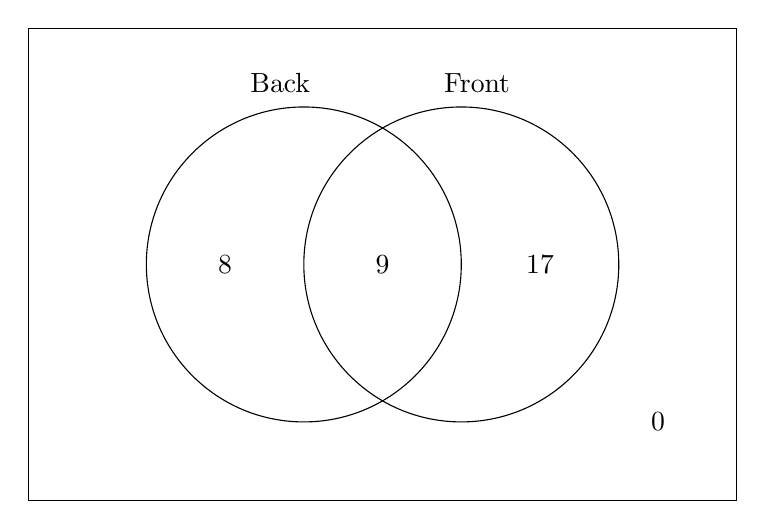
\begin{tikzpicture}
	\draw (0,0) rectangle (9,6);
	\draw (3.5,3) circle (2);
	\draw (5.5,3) circle (2);
	
	\node at (3.2,5.3) {Back};
	\node at (5.7,5.3) {Front}; 
	
	\node at (2.5,3) {8};
	\node at (4.5,3) {9};
	\node at (6.5,3) {17};
	\node at (8,1) {0};
	\end{tikzpicture}
	\]



\newpage



% Problem 2
\problem{10} You can either take the `short' way to work or the `long' way. The short way has less distance but you are more likely to hit traffic. If you take the short way, there is a 10\% chance that you will be late to work. If you take the long way, there is only a 5\% chance that you will be late to work. You take the short way to work 70\% of the time.
	\begin{enumerate}[(a)]
	\item What is the probability that you are on-time for work?
	\item What is the probability that you are late to work?
	\item What is the probability that you are on-time for work or took the long way to work?
	\item If you were late to work, what is the probability that you took the long way there?
	\end{enumerate} \pspace

\sol 
\begin{enumerate}[(a)]
\item 
	\[
	P(\text{on-time})= 0.63 + 0.285= 0.915
	\]

\item 
	\[
	P(\text{late})= 0.07 + 0.015= 0.085
	\]

\item 
	\[
	P(\text{on-time or long way})= 0.63 + 0.015 + 0.285= 0.93
	\]

\item 
	\[
	P(\text{long way} \;|\; \text{late})= \dfrac{0.015}{0.07 + 0.015}= \dfrac{0.015}{0.085}= 0.1765
	\]
\end{enumerate} \vfill

		\[
		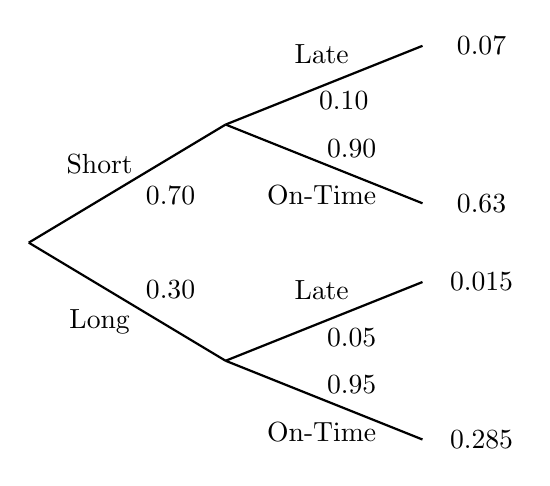
\begin{tikzpicture}[scale= 1.0]
		\def\FirstUpLabel{Short}
		\def\FirstDownLabel{Long}
		\def\SecondUpLabel{Late}
		\def\SecondDownLabel{On-Time}
		\def\Up{$0.70$}
		\def\Down{$0.30$}
		\def\UpUp{$0.10$}
		\def\UpDown{$0.90$}
		\def\DownUp{$0.05$}
		\def\DownDown{$0.95$}
		\def\first{$0.07$}
		\def\second{$0.63$}
		\def\third{$0.015$}
		\def\fourth{$0.285$}
		
		\node at (0.9,1) {\FirstUpLabel};	
		\node at (0.9,-1) {\FirstDownLabel};	
		\node at (1.8,0.6) {\Up};
		\node at (1.8,-0.6) {\Down};
		\draw[thick] (0,0) -- (2.5,1.5);
		\draw[thick] (0,0) -- (2.5,-1.5);
		
		\node at (3.72,2.4) {\SecondUpLabel};
		\node at (3.72,0.6) {\SecondDownLabel};
		\node at (4,1.8) {\UpUp};
		\node at (4.1,1.2) {\UpDown};
		\node at (5.75,2.5) {\first};
		\node at (5.75,0.5) {\second};
		\draw[thick] (2.5,1.5) -- (5,2.5);
		\draw[thick] (2.5,1.5) -- (5,0.5);

		\node at (3.72,-0.6) {\SecondUpLabel};
		\node at (3.72,-2.4) {\SecondDownLabel};
		\node at (4.1,-1.2) {\DownUp};
		\node at (4.1,-1.8) {\DownDown};
		\node at (5.75,-0.5) {\third};	
		\node at (5.75,-2.5) {\fourth};	
		\draw[thick] (2.5,-1.5) -- (5,-0.5);
		\draw[thick] (2.5,-1.5) -- (5,-2.5);
		\end{tikzpicture}
		\]


\end{document}